Яни является любительницей птиц. С тех пор как она прочла о протоколе \textit{IP over Avian Carriers} (IPoAC), она провела много времени, дрессируя стаю умных попугаев для передачи сообщений на дальние расстояния.

Яни мечтает использовать своих птиц, чтобы передать сообщение $M$ в очень далекую страну. Её сообщение $M$ является последовательностью из $N$ (не обязательно различных) целых
чисел, каждое от $0$ до $255$ включительно. У Яни есть $K$ специально натренированных
попугаев. Все попугаи выглядят одинаково, Яни их не различает. Каждая птица может
запоминать одно целое число от $0$ до $R$ \textit{включительно}.

Вначале Яни использовала простую схему: чтобы послать сообщение, Яни аккуратно
выпускала птиц из клетки одну за другой. Перед тем как каждая из птиц улетала, Яни учила
птицу очередному числу из последовательности, образующей сообщение. К сожалению, эта
схема не срабатывала. Оказалось, что все птицы прилетают в пункт назначения, но они не
обязательно прилетают в том же порядке, в котором они улетали. Используя эту схему, Яни
могла восстановить все числа, которые она отправляла, но у неѐ не получалось расположить
их в правильном порядке.

Чтобы исполнить мечту, Яни нужна лучшая схема, и для этого Яни нуждается в вашей
помощи. Имея сообщение $M$, она планирует выпускать птиц одну за другой, как и раньше.
Необходимо написать программу, которая будет выполнять две отдельные операции:
\begin{itemize}
\item Во-первых, программа должна читать сообщение $M$ и преобразовывать его в
последовательность из не более чем $K$ целых чисел от $0$ до $R$, которым Яни сможет
обучить птиц.
\item Во-вторых, программа должна читать последовательность из целых чисел от $0$ до $R$,
получаемых по мере достижения птицами пункта назначения, после чего
преобразовать их назад в исходное сообщение $M$.
\end{itemize}
Гарантируется, что все попугаи всегда прилетают в пункт назначения и что каждый из них
помнит выученное им число. Яни еще раз напоминает, что попугаи могут прилетать в
произвольном порядке. Необходимо обратить внимание, что у Яни есть только $K$ попугаев, то
есть, последовательность целых чисел от $0$ до $R$, в которую преобразуется сообщение,
должна содержать не более $K$ целых чисел.

Ваше задание -- написать две отдельные процедуры. Одна из них будет использоваться при отправлении (encoder), а другая при получении (decoder).

Весь процесс показан на рисунке ниже.

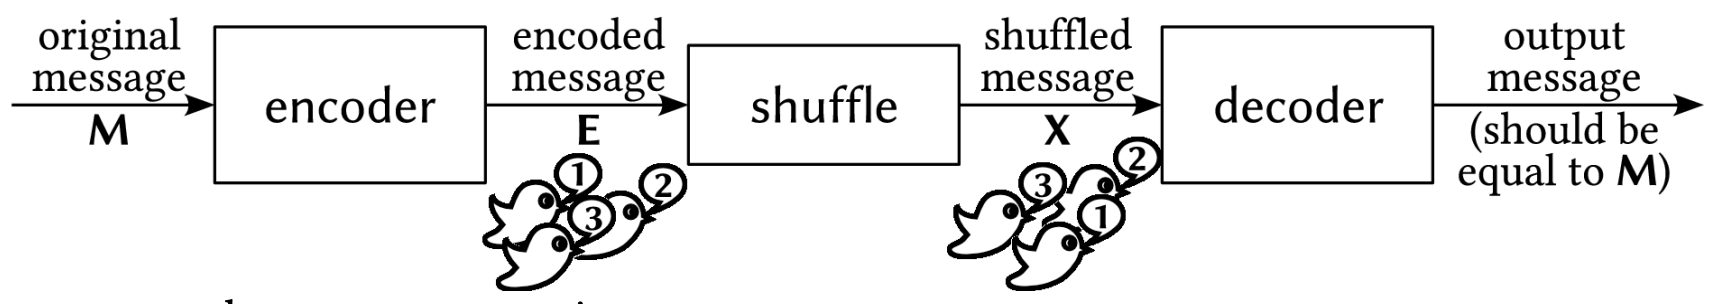
\includegraphics[width=175mm]{parrots1.png}

Напишите две следующие процедуры:
\begin{itemize}
\item Процедуру \t{encode(N,M)}, которой передаются следующие параметры:
\begin{itemize}
\item $N$~--- длина сообщения.
\item $M$~--- одномерный массив из $N$ целых чисел, которые представляют сообщение.
Гарантируется, что $0 \leq M[i] \leq 255$ для $0 \leq i < N$.
\end{itemize}
Эта процедура должна кодировать сообщение $M$ в последовательность, которая будет
пересылаться с помощью попугаев и которая состоит из целых чисел от $0$ до $R$
включительно. Чтобы сообщить эту последовательность, процедура \t{encode} должна
вызывать процедуру \t{send(a)} для каждого целого числа $a$, которому вы хотите обучить
очередную птицу.
\item Процедуру \t{decode(N,L,X)}, которой передаются следующие параметры:
\begin{itemize}
\item $N$~--- длина исходного сообщения.
\item $L$~--- длина полученного сообщения (количество отправленных птиц).
\item $X$~--- одномерный массив из $L$ целых чисел, которые были получены. Числа
$X[i]$ для $0 \leq i < L$ являются точно теми же числами, которые сгенерировала
процедура \t{encode}, но они, возможно, расположены в другом порядке. 
\end{itemize}
Эта процедура должна восстановить исходное сообщение. Чтобы сообщить его,
процедура \t{decode} должна вызывать процедуру \t{output(b)} для каждого целого числа $b$
из расшифрованного сообщения в том порядке, в котором они образуют исходное
сообщение.
\end{itemize}
Необходимо обратить внимание, что значения $R$ и $K$ не передаются как входные параметры
(см. описание подзадач ниже).

Чтобы правильно решать определенную подзадачу, ваши процедуры должны удовлетворять
следующим условиям:
\begin{itemize}
\item Все целые числа, отправляемые процедурой \t{encode} с помощью процедуры \t{send},
должны быть в диапазоне, указанном в подзадаче.
\item Количество вызовов процедуры \t{send}, которые делает ваша процедура \t{encode}, не
должно превышать предельное значение $K$ указанное в подзадаче. Необходимо
обратить внимание, что значение $K$ зависит от длины сообщения.
\item Процедура \t{decode} должна правильно восстанавливать исходное сообщение $M$ и
вызывать процедуру \t{output(b)} ровно $N$ раз со значениями $b$, равными числам $M[0], M[1], \dots, M[N-1]$.
\end{itemize}
В последней подзадаче баллы, получаемые в результате оценивания, зависят от отношения
между длинами закодированного и исходного сообщений.